%!TEX program = xelatex
%%
%% This is file `mcmthesis-demo.tex',
%% generated with the docstrip utility.
%%
%% The original source files were:
%%
%% mcmthesis.dtx  (with options: `demo')
%% !Mode:: "TeX:UTF-8"
%% --
%% This is a generated file.
%% 
%% Copyright (C) 2010 -- 2015 by latexstudio
%%       2014 -- 2019 by Liam Huang
%%       2019 -- present by latexstudio.net
%% 
%% License: The LaTeX Project Public License 1.3c
%% 
%% The Current Maintainer of this work is latexstudio.net.
%% 
\documentclass[UTF8, fontset=windows]{mcmthesis}
 %\documentclass[CTeX = true]{mcmthesis}  % 当使用 CTeX 套装时请注释上一行使用该行的设置
\mcmsetup{tstyle=\color{red}\bfseries,%修改题号,队号的颜色和加粗显示,黑色可以修改为 black
        tcn = 武泽恺, problem = E, %修改队号,参赛题号
        sheet = true, titleinsheet = true, keywordsinsheet = true,%修改sheet显示信息
        titlepage = false, abstract = true}

  %四款字体可以选择
  %\usepackage{times}
  \usepackage{newtxtext,newtxmath}
  \usepackage{fix-cm} % Ensure consistent font sizes
  %\usepackage{palatino}
  %\usepackage{txfonts}
  \usepackage[UTF8, nocap]{ctex}

\bibliographystyle{plain}

\usepackage{indentfirst}  %首行缩进,注释掉,首行就不再缩进。
\usepackage{lipsum}
\title{\textbf{全球塑料危机治理方案:MSPWR与PWRAM模型}}
\author{\small \href{https://www.latexstudio.net/}
  {\includegraphics[width=7cm]{mcmthesis-logo}}}
\date{\today} 
\begin{document}
\begin{abstract}
\par 自1950年代以来,全球塑料总量已经超过了8300万吨。虽然塑料为我们的生活带来了极大的便利,但也在无时不刻的破坏着我们的环境。为了缓解这一全球危机,我们的研究提出了两个数学模型(MSPWR和PWRAM),希望能够为全球性的治理方案提供一定的数学依据。

首先,我们构建了\textbf{MSPWR模型},该模型基于可降解塑料产量、甲烷和二氧化碳排放等数据,可以用于精确估计能够安全减轻的一次性塑料产品浪费的最大量,并保证了不会进一步破环环境。但是,不同的国家会因为一些复杂的政治、经济等因素而影响其塑料制品浪费减少能力。因此,我们建立了\textbf{PWRAM模型},用于综合评量一个国家或地区的塑料制品浪费减少能力。我们通过\textbf{最小-最大归一化}处理各个国家或地区的HDI、WGI、GII、EPI数据,利用\textbf{熵权法}计算了它们的PWRAM水平,给出了我们的评量结果。为全球一次性或一次性塑料产品的使用可达到的最低水平,我们全球发展中国家设定了明确的目标,并提出了一系列解决方案,包括提升WGI和GII水平,并以巴西为例进行了具体的分析,期望在30年内使巴西的PWRAM水平达到0.7的目标水平。我们还分析了实现这一目标对塑料业、生态环境和人类生活的影响。最终,为了解决公平性问题,我们强调了危机与各个国家的相关性,敦促发达国家承担更多的责任,共同推动全球塑料垃圾治理事业的发展。

\textbf{关键词:}塑料垃圾;环境保护;全球治理

Since the 1950s, the total amount of plastic produced worldwide has exceeded 83 million tons. Although plastics have brought great convenience to our lives, they have also harmed our environment. To address this global issue, our study proposes two models (MSPWR and PWRAM), which aims to provide a mathematical foundation for global governance strategies.

First, we developed the MSPWR model, accurately estimating the maximum amount of single-use plastic waste that can be safely reduced, which is based on data such as the amount of biodegradable plastic production, methane, and carbon dioxide emissions. This ensures that reductions will not further damage the environment. However, the ability to reduce plastic waste varies across countries due to political, economic, and other factors. To address this issue, we established the PWRAM model to assess a country or region’s ability to reduce plastic waste. By normalizing HDI, WGI, GII, and EPI data from various countries and regions, we calculated their PWRAM levels with the entropy weight method.

To achieve the lowest possible level of single-use plastic consumption globally, we set a target for developing countries and proposed feasible solutions, including improving WGI and GII levels. We used Brazil as a studying case and analyzed the feasibility of achieving a PWRAM level of 0.7 within 30 years. Furthermore, we assessed the impact of reaching this target on the plastic industry, the ecological environment, and human life. Finally, to address inequality issues, we emphasized the strong relationship between all nations, urging developed countries to take greater responsibility and make more efforts to manage plastic waste.

\begin{keywords}
Plastic waste; Environmental protection; Global governance
\end{keywords}
\end{abstract}
\maketitle
%% Generate the Table of Contents, if it's needed.
\tableofcontents
\newpage
%%
%% Generate the Memorandum, if it's needed.
% \memoto{\LaTeX{}studio}
% \memofrom{Liam Huang}
% \memosubject{Happy \TeX{}ing!}
% \memodate{\today}
% \memologo{\LARGE I'm pretending to be a LOGO!}
% \begin{memo}[Memorandum]
%   \lipsum[1-3]
% \end{memo}
%%
\section{介绍}
\subsection{问题背景}

在如今的社会中,塑料制品已经成为人们生活中不可或缺的一部分。自1950年代以来,食品包装、消费品、医疗设备和建筑业等工业产业快速发展,塑料制造业的发展速度也呈指数增长。如图\ref{fig:circle1}所示,自1950年以来,全球生产的塑料总量已经超过了8300万吨,其中约30\%的塑料被用于一次性塑料制品的生产。尽管一次性塑料制品的使用方便,但由于其使用后难以处理,只有9\%的塑料被回收利用,大部分塑料被焚烧、填埋或倒入海洋。据估计,仅2010年一年内进入海洋的塑料废物就高达400到1200万吨 \cite{geyer2017production}。由于塑料需要数百年才能降解,这些废弃物对环境造成了严重的污染。如果不采取措施,到2050年,海洋中的塑料垃圾将超过鱼类的总重量 \cite{jambeck2015plastic}。由于大量的塑料废弃物进入海洋生物体内,不仅破坏了海洋生态系统,食物链中的塑料微粒同时也会最终进入人类食物链,对人类健康造成威胁。

\begin{figure}[h]
\centering
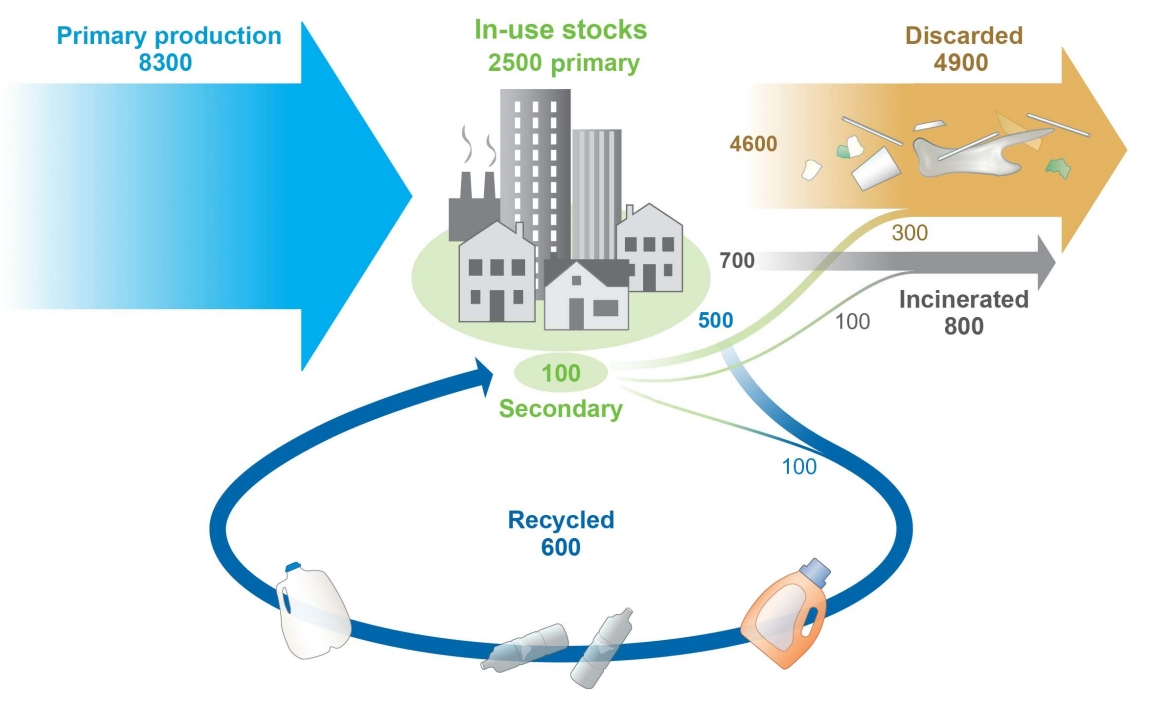
\includegraphics[width=0.8\textwidth]{circle1}
\caption{自1950年以来全球塑料的生产、使用及处理。 \cite{geyer2017production}} 
\label{fig:circle1}
\end{figure}

因此,减少一次性塑料制品的浪费,提高塑料回收利用率,已经成为全球范围内的热门话题。

\subsection{问题复述}

我们通过建立数学模型来解决以下问题:

\begin{itemize}
  \item 我们需要建立一个模型以估算可以安全减轻的一次性或一次性使用的塑料产品浪费的最大量,而不会造成进一步的环境破坏。
  \item 我们需要讨论可以减少塑料垃圾以达到环境安全水平的程度。
  \item 我们需要借助模型来为全球一次性塑料产品垃圾可减少到的最低水平设定一个目标值,并讨论达到这一水平的影响。
  \item 我们需要讨论如何在全球范围内推动我们的解决方案,以及是否会出现一些潜在的公平问题。
\end{itemize}

\subsection{我们的工作}

在本文中,我们首先建立了一个一次性塑料制品浪费最大化减少的模型 (Maximum Single-use Plastic Waste Reduction Model, MSPWR) ,来估算每年一个国家可以安全减轻的一次性塑料产品浪费的最大量。然后,我们建立了一个塑料制品浪费减少能力模型 (Plastic Waste Reduction Ability Model, PWRAM) ,来估算一个国家或地区的塑料制品浪费减少能力。随后,我们为全球一次性塑料产品垃圾可减少到的最低水平设定了一个目标值,即PWRAM水平达到0.7。我们结合了巴西的具体数据进行了分析,预测通过国内和国际共同作用下可以在30年内实现这一水平。同时,我们还讨论了达到这一水平对塑料业、生态环境和人类生活的影响。最后,由于不同的发达国家与发展中国家的PWRAM平均水平差距较大,我们讨论了可能出现的一些潜在的公平问题,并给出了通过建立多边合作来实现合作共赢的解决方案。

\section{假设}

我们的模型基于以下假设:

\begin{itemize}
  \item 由于所有的数据都是从公开的网络数据集中获取的,我们假设这些数据是准确的,这是因为这些数据集是由专业机构、政府部门或者学术研究机构发布的,具有较高的可信度。
  \item 我们假设所有的塑料制品在使用后,一部分会被回收利用,剩余的部分会被当作废物,通过填埋或者焚烧处理,仅通过这三种方式进行处理。这一点方便我们对塑料废物的处理进行估算。
  \item 我们假设环境承载能力可以在人力干预下随时间逐渐变化。一般情况下,如果环境的负荷超过了环境承载能力,那么环境会受到负反馈破坏,进一步降低环境承载能力。但是,如果我们采取了有效的措施,那么环境承载能力可以逐渐恢复甚至提高。
  \item 我们假设各个国家和地区积极应对塑料废物的处理问题,会采取有效的措施来减少塑料废物的产生。
\end{itemize}

\section{记号及定义}

我们在模型中使用的符号和定义展示在表\ref{tab:notation}中。

\begin{table}[h]
\centering
\begin{tabular}{cc}
\toprule
符号 & 定义\\
\midrule
$P$ & 每年生产的塑料制品总量\\
$P_s$ & 每年生产的一次性塑料制品总量\\
$q_s$ & 一次性塑料制品的比例\\
$W_s$ & 每年处理的塑料废物总量\\
$R_s$ & 每年回收利用的一次性塑料总量\\
$L_s$ & 每年填埋的一次性塑料总量\\
$I_s$ & 每年焚烧的一次性塑料总量\\
$M_s$ & 每年随意丢弃的一次性塑料总量\\
$V_s$ & 每年有效处理的一次性塑料总量\\
$p_1$ & 回收利用的比例\\
$p_2$ & 填埋的比例\\
$p_3$ & 焚烧的比例\\
$\dot{E}_{CH_4}$ & 填埋一吨塑料废物产生的甲烷气体总量\\
$E_{CH_4}^c$ & 某国家$c$全年计划排放的甲烷气体总量\\
$L$ & 填埋场所排放的甲烷气体总量\\
$p_{lf}$ & 填埋场所排放的甲烷气体总量占全国排放总量的比例\\
$P_{bio}$ & 生物可降解塑料的产量\\
$L_{max}$ & 填埋塑料的理论最大量\\
$\dot{E}_{CO_2}$ & 焚烧一吨塑料废物产生的二氧化碳总量\\
$E_{CO_2}^c$ & 某国家$c$全年计划排放的二氧化碳总量\\
$p_{inc}$ & 工业焚烧设施排放的二氧化碳总量占全国排放总量的比例\\
$I$ & 工业焚烧设施排放的二氧化碳总量\\
$x_i^j$ & 第$i$个国家或地区的第$j$个指标的值\\
$y_i^j$ & 第$i$个国家或地区的第$j$个指标的归一化值\\
$I_j$ & 第$j$个国家的综合指标,即PWRAM水平\\
$w_i$ & 第$i$个指标的权重\\
$H_i$ & 第$i$个指标的熵值\\
$p_{ij}$ & 第$i$个指标的第$j$个国家的数据中的占比\\
\bottomrule
\end{tabular}
\caption{本文所使用的符号及其定义}
\label{tab:notation}
\end{table}

\section{塑料制品浪费最大化减少模型}

\subsection{MSPWR模型}

在本节中,我们建立了一个一次性塑料制品浪费最大化减少的模型 (Maximum Single-use Plastic Waste Reduction Model, MSPWR),来估算每年生产的一次性塑料制品总量、每年处理的塑料废物总量,以及可以安全减轻的一次性塑料产品浪费的最大量。

在塑料制品当中,塑料包装是最主要的一种。图\ref{fig:pld}中,数据\cite{geyer2017production}用对数正态分布来拟合了塑料使用寿命的分布。在这个分布中,塑料包装的使用寿命主要集中在一年以内,其余的塑料制品的使用寿命主要集中在3年以上。因此,我们可以将前者定义为“一次性塑料制品”,将后者定义为“非一次性塑料制品”。根据题目要求,在本模型中,我们主要关注一次性塑料制品的浪费。

\begin{figure}[h]
\centering
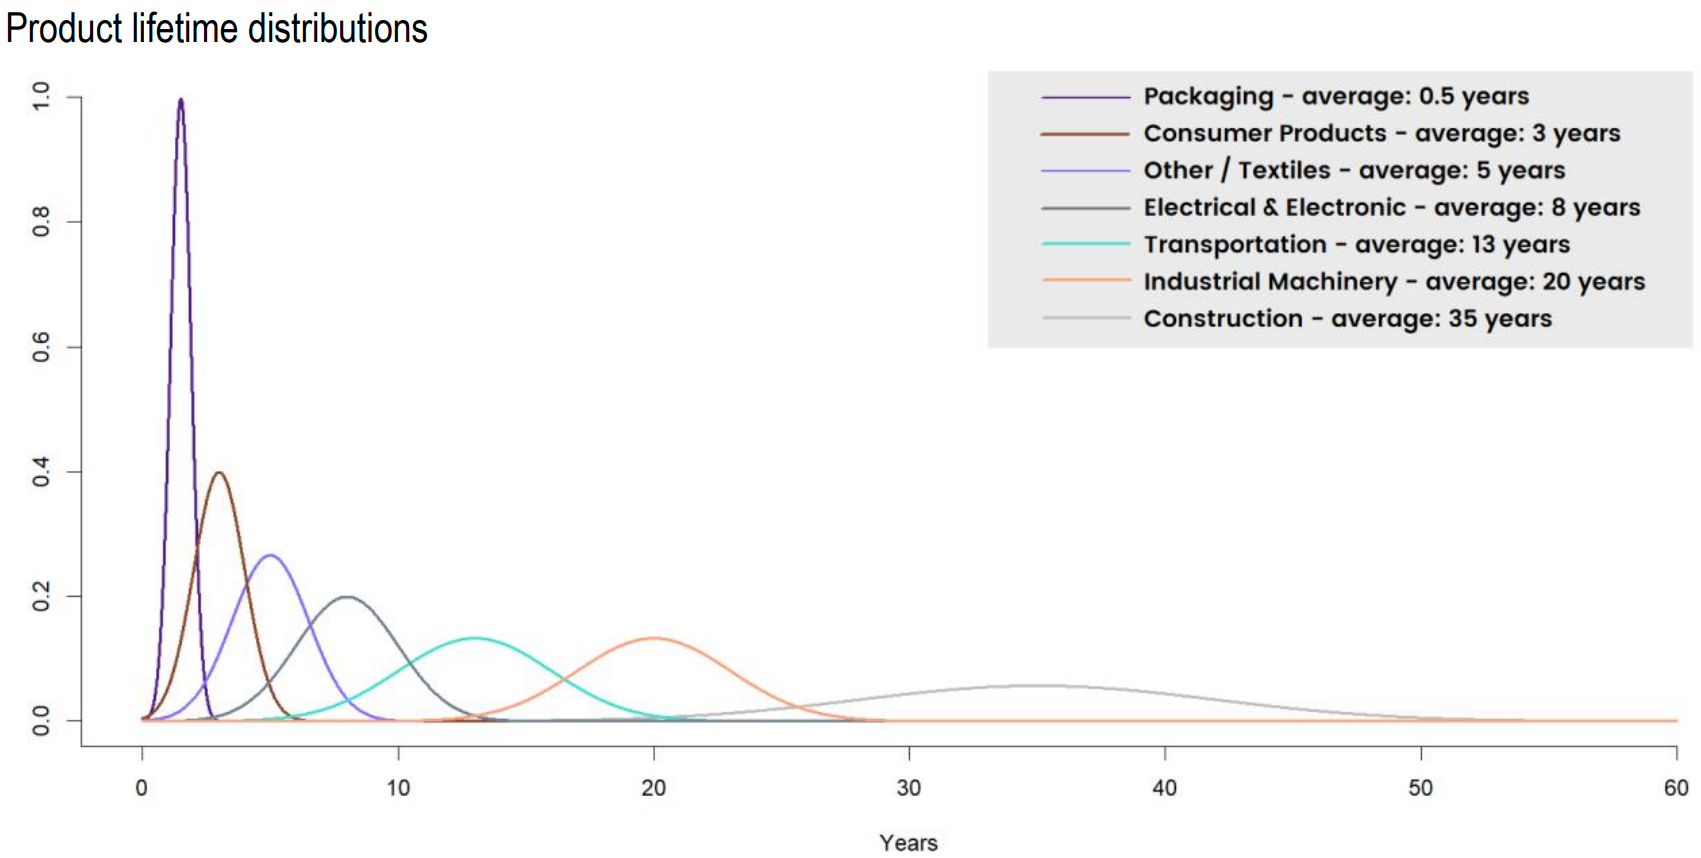
\includegraphics[width=0.8\textwidth]{plds}
\caption{塑料制品的生命周期}
\label{fig:pld}
\end{figure}

我们首先假设每年生产制品总量为$P$,假设一次性塑料制品的比例为$q_s$。因此,每年生产的一次性塑料总量为$P_s$,那么,

\begin{equation}
P_s = P \times q_s
\end{equation}

\begin{figure}[h]
\centering
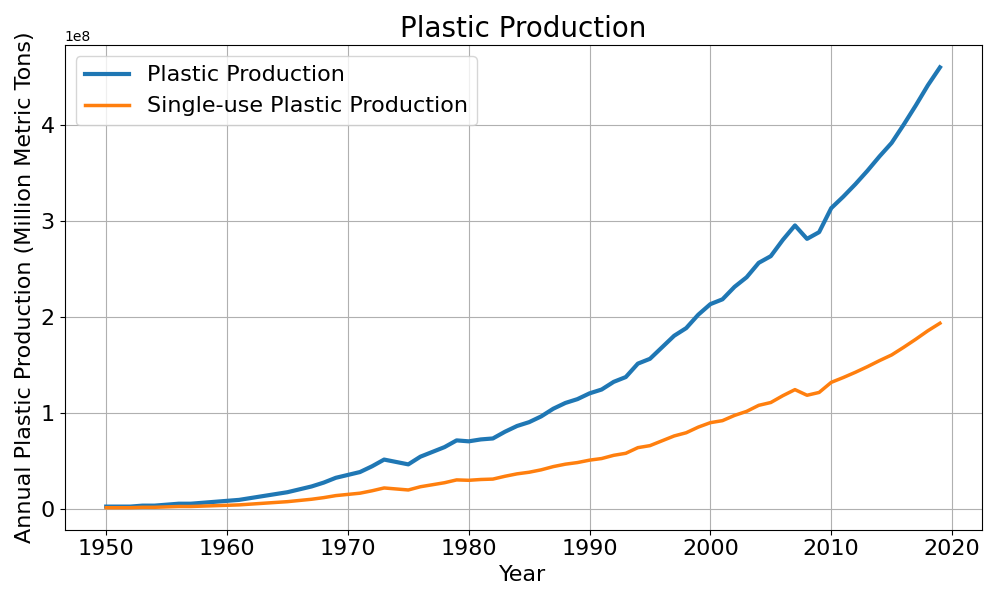
\includegraphics[width=0.8\textwidth]{production_amount}
\caption{全球塑料制品的生产总量}
\label{fig:production_amount}
\end{figure}

在图\ref{fig:circle1}中,我们已经看到了全球塑料的生产、使用和处理的情况。其中,处理方式主要包括三种:回收利用、填埋和焚烧。我们假设每年处理的一次性塑料废物总量为$W_s$,其中回收利用的部分为$R_s$,填埋的部分为$L_s$,工业焚烧的部分为$I_s$。然而,尽管大部分的塑料都能够被有效处理,仍有一部分塑料会被随意丢弃(Mismanaged Plastic Waste)。由于政策的不完善、管理的不善,这部分塑料会被丢弃在不受控制的垃圾场、露天焚烧、\textbf{倾倒海洋}或泄漏到环境中。这部分为$M_s$。因此,

\begin{equation}
W_s = R_s + L_s + I_s + M_s
\end{equation}

\begin{figure}
\centering
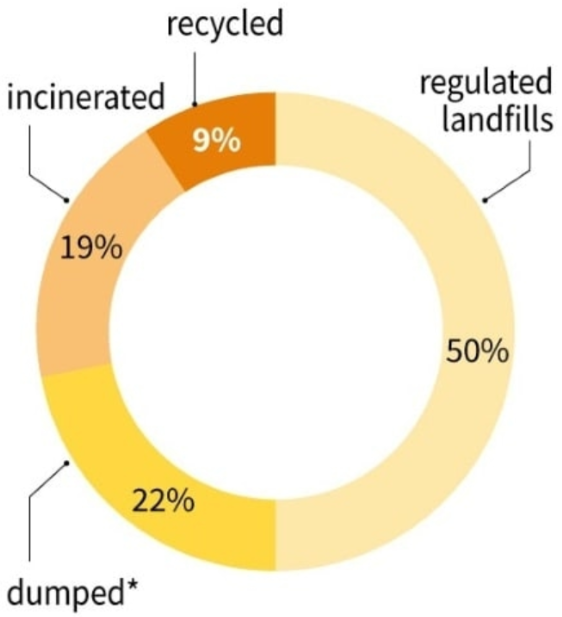
\includegraphics[width=0.4\textwidth]{proportion}
\caption{全球塑料废物的处理比例}
\label{fig:proportion}
\end{figure}

因此,我们定义了有效处理的一次性塑料废物总量$V_s$,为使$V_s$达到最大值,我们有,

\begin{equation}
\max V_s = \max (W_s - M_s) = \max (R_s + L_s + I_s)
\end{equation}

我们需要需要分别最大化$R_s$、$L_s$和$I_s$。方便起见,我们假设不同处理方式所处理的一次性塑料废物比例是固定的,分别为$p_1$、$p_2$和$p_3$。

\subsubsection{回收利用最大化}

工业界对于塑料回收利用的技术已经相对成熟,主要包括机械回收、化学回收和能量回收\cite{hopewell2009plastics}。然而,由于塑料的种类繁多,不同种类的塑料需要不同的回收技术,因此回收利用的效率并不高。同时,无论是机械回收还是化学回收,都需要大量的能源和资源,因此回收利用的成本也较高。根据数据显示\cite{annexcompose},2019年全球回收利用的塑料总量约为3150万吨,仅占全球生产的9\%。

每年可以最大化回收利用的一次性塑料总量$R_s$,取决于不同的回收利用技术、回收政策和回收设施的建设。如前文所定义的,回收利用的比例为$p_1$,即回收利用的塑料总量与生产的塑料总量的比值。因此我们可以得到,

\begin{equation}
R_s = P_s \times p_1
\end{equation}

根据这个公式,我们可以估算出每年回收利用的一次性塑料总量。

\subsubsection{陆地填埋最大化}

陆地填埋是目前处理塑料废物最常用的方式之一。填埋的优点是处理方便、成本低廉,但缺点是占用大量的土地资源,同时填埋的塑料废物会随着时间的推移逐渐分解,产生大量的甲烷气体,对环境造成污染。根据数据显示\cite{annexcompose},全球每年填埋的塑料总量约为1.75亿吨,占全球生产的50\%。

在陆地填埋过程中,主要发生了厌氧发酵反应,产生了大量的甲烷气体。这个过程可以用以下化学方程式表示:

\begin{equation}
(\text{C}_3\text{H}_4\text{O}_2)_n + \text{H}_2\text{O} \xrightarrow{\text{Enzymes}} \text{CH}_4 + \text{H}_2\text{O}
\end{equation}

因此,我们可以通过考虑甲烷气体的排放量来评估陆地填埋的塑料废物的最大量。我们假设填埋每吨塑料废物产生的甲烷气体总量为$\dot{E}_{CH_4}$,某国家$c$全年计划排放的甲烷气体总量为${E}^{c}_{CH_4}$,陆地填埋场所排放的甲烷气体总量占全国排放总量的比例为$p_{lf}$。因此,我们可以得到,

\begin{equation}
L = \frac{{E}^{c}_{CH_4} \times p_{lf}}{\dot{E}_{CH_4}}
\end{equation}


然而,并不是所有的塑料废物都是生物可降解的。从保护环境的角度来考虑,我们认为被用于陆地填埋的废物塑料均是生物可降解的,这会受到实际生物可降解塑料产量的限制。我们假设生物可降解塑料的产量为$P_{bio}$,那么,

\begin{equation}
L_{max} = \min(L, P_{bio})
\end{equation}

对于一次性塑料废物的填埋,我们有,

\begin{equation}
L_s = L_{max} \times q_s
\end{equation}

通过这个公式,我们可以估算出每年填埋的一次性塑料总量。

\subsubsection{工业焚烧最大化}

工业焚烧是目前处理塑料废物的另一种常用方式。焚烧的优点是处理方便、占地面积小,同时焚烧的塑料废物可以转化为能量,可以用于发电。然而,焚烧的缺点是会产生大量的二氧化碳和其他有害气体,对环境造成污染。根据数据显示\cite{annexcompose},全球每年焚烧的塑料总量约为0.67亿吨,占全球生产的19\%。

在全球范围内,采用焚烧的塑料废物主要是通过工业焚烧设施进行处理。这些设施通常配备有高效的过滤装置,可以有效减少有害气体的排放。因此,我们可以通过考虑焚烧设施的$CO_2$排放量来评估焚烧的塑料废物的最大量。我们假设焚烧每吨塑料废物产生的二氧化碳总量为$\dot{E}_{CO_2}$,某国家$c$全年计划排放的二氧化碳总量为${E}^{c}_{CO_2}$,工业焚烧设施排放的二氧化碳总量占全国排放总量的比例为$p_{inc}$。因此,我们可以得到,

\begin{equation}
I = \frac{{E}^{c}_{CO_2} \times p_{inc}}{\dot{E}_{CO_2}}
\end{equation}

那么,一次性塑料废物的焚烧总量为,

\begin{equation}
I_s = I \times q_s
\end{equation}

通过这个公式,我们可以估算出每年焚烧的一次性塑料总量。

\subsubsection{应用MSPWR模型}

借助我们的MSPWR模型,我们可以利用每年国家的相关数据来估算可以安全减轻的一次性塑料产品浪费的最大量。

我们以2010年的中国为例。数据显示\cite{owid-plastic-pollution},2010年中国生产的塑料总量为44,325,900吨,其中一次性塑料制品的比例为42\%。同时,2010年中国回收的塑料比例为9\%,我们可以计算出$R_s$的值。根据IPCC所提供的信息\cite{ipccworkinggroupii2022climate},填埋一吨塑料废物产生的甲烷气体总量为0.046 吨二氧化碳当量,结合UNFCCC给出的信息\cite{china_third_national_communication},可以得到2010年中国所计划排放的甲烷气体总量为1,163,000,000吨二氧化碳当量,计划排放的二氧化碳总量为7,678,000,000吨,废弃物填埋场所排放的甲烷约占7.9\%,工业焚烧设施排放的二氧化碳约占0.104\%,我们可以计算出$L$、$I$的值。根据水清木华研究所提供的近年来国内可降解塑料信息\cite{biodegradable2010},我们可以通过拟合二次曲线来估算出2010年中国的生物可降解塑料产量为225,000吨,代码见附录\ref{sec:fit}。结合这些数据信息,我们可以得到,

\begin{equation}
\left\{
\begin{aligned}
P_s &= 44,325,900 \times 42\% = 18,616,878\\
R_s &= 18,616,878 \times 9\% = 1,675,513\\
L_s &= \min(\frac{1,163,000,000 \times 7.9\%}{0.046}, 225,000) \times 42\% = 94,500\\
I_s &= \frac{7,678,000,000 \times 0.104\%}{2.9} \times 42\% = 1,156,465
\end{aligned}
\right.
\end{equation}

因此,我们可以得到2010年中国可以安全减轻的一次性塑料产品浪费的最大量为$V_s = 1,675,513 + 94,500 + 1,156,465 = 2,926,478$吨。

\subsection{塑料制品浪费减少能力模型}

上节中,我们建立了一个模型来估算可以安全减轻的一次性塑料产品浪费的最大量。然而,在现实中,一个国家或地区的能够减轻的塑料产品浪费量是有限的,这取决于其自身的减排能力。因此,我们需要建立一个模型来估算一个国家或地区的塑料制品浪费减少能力,即塑料制品浪费减少能力模型(Plastic Waste Reduction Ability Model, PWRAM)。

\subsubsection{模型建立}

在现实生活中,有多种因素会影响一个国家或地区的塑料制品浪费减少能力,如塑料新产品的研发、塑料处理技术的提升、塑料使用对公民生活的影响、环境保护意识的不同、环境承载能力的差异、政府的政策支持等等。为了能够综合考虑各个地区的具体制约因素,我们认真选取了以下几个\textbf{全球范围内认可度较高的指标}作为我们模型的输入参数:

\begin{itemize}
  \item 经济水平:人类发展指数(Human Development Index, HDI)\cite{UNDP_HDI} 是联合国开发计划署用于衡量一个国家或地区的人类发展水平的综合指标。HDI的计算包括三个维度:健康、教育和生活水平。HDI的取值范围为0到1,数值越大表示人类发展水平越高。如果一个国家或地区的HDI值较高,那么人们接受价格更高的环保产品的意愿可能更强,从而减少塑料制品的使用。
  \item 政治水平:全球治理指标(Global Governance Index, WGI)\cite{WorldBank_WGI} 是由世界银行发布的用于衡量一个国家或地区的全球治理水平的综合指标。WGI的计算包括多个维度:政治参与度、政治稳定度、政府效能、政府腐败管控能力、政府法制能力等等。WGI的各项指标取值范围为0到100,我们取各个指标平均值来表示其综合治理水平,数值越大表示治理水平越高。如果一个国家或地区的WGI值较高,那么政府所推出的环保政策可能更加有效,从而减少一次性塑料制品的消耗。
  \item 科技水平:全球创新指数(Global Innovation Index, GII)\cite{WIPO_GII} 是世界知识产权组织用于衡量一个国家或地区的创新能力的综合指标。GII的计算包括多个维度:创新环境、创新投入、创新产出等。GII的取值范围为0到100,数值越大表示创新能力越强。如果一个国家或地区的GII值较高,那么可能会有更多的创新技术用于塑料制品的替代,从而降低对塑料制品的需求。
  \item 环境水平:环境绩效指数(Environmental Performance Index, EPI)\cite{EPI_Report} 是由耶鲁大学和哥伦比亚大学联合开发的用于衡量一个国家或地区的环境绩效的综合指标。EPI的计算包括多个维度:空气质量、水质、生态系统健康等。EPI的取值范围为0到100,数值越大表示环境绩效越好。如果一个国家或地区的EPI值较高,那么会有更高的环境承载能力,从而可以更好地处理塑料废物。
\end{itemize}

我们分别用$x_{HDI}$、$x_{WGI}$、$x_{GII}$、$x_{EPI}$来表示一个国家或地区的HDI、WGI、GII、EPI的数值。由于这些指标的取值范围不同,我们需要对其进行归一化处理,使其在0到1之间。我们采用最小-最大归一化的方法,即,

\begin{equation}
y_{i}^{j} = \frac{x_{i}^{j} - \min(x_{i})}{\max(x_{i}) - \min(x_{i})}
\end{equation}

其中,$x_i^j$表示第$j$个国家或地区的第$i$个指标的原始数值,$\min(x_i)$和$\max(x_i)$分别表示第$i$个指标的最小值和最大值,$y_i^j$表示第$j$个国家或地区的第$i$个指标的归一化数值。通过这个方法,我们可以将不同国家或地区的HDI、WGI、GII、EPI的数值转化为0到1之间的数值。

为了能够将这些指标综合考虑,我们可以采用线性加权模型或者熵权法模型。在这里,我们采用熵权法模型,因为熵权法模型可以通过自适应各个指标之间的相关性来得到其权重。熵权法模型的计算公式如下:

\begin{equation}
I_j = \sum_{i=1}^{4} w_i \times y_i^j
\end{equation}

其中,$w_i$表示第$i$个指标的权重,$y_i^j$表示第$j$个国家或地区的第$i$个指标的归一化数值,$I_j$表示第$j$个国家或地区的综合指标。我们通过如下的公式来计算权重:

\begin{equation}
w_i = \frac{1 - H_i}{\sum_{j=1}^{4} (1 - H_j)}
\end{equation}

其中,$H_i$表示第$i$个指标的信息熵,计算公式如下:

\begin{equation}
H_i = k \times \sum_{j=1}^{n} p_{ij} \times \ln p_{ij}
\end{equation}

其中,$p_{ij}$表示第$i$个指标在第$j$个国家的占比,$k=-\frac{1}{\ln n}$为标准化系数,$n$为国家或地区的数量。结合上述公式,我们可以得到一个国家或地区的综合指标$I_j$。

\subsubsection{应用PWRAM模型}

借助我们的PWRAM模型,我们可以利用全球范围内的HDI、WGI、GII、EPI的数据来估算一个国家或地区的塑料制品浪费减少能力,即$I_j$的数值,数值越大表示一个国家或地区的塑料制品浪费减少能力越强。

我们以全球范围内的15个不同的国家或地区作为分析对象。我们选择了四个指标的最新数据,同时保证这些数据均来自同一年份,以保证数据的可比性。通过查找相关资料后,我们发现2022年的HDI\footnote{\url{https://hdr.undp.org/system/files/documents/global-report-document/hdr2023-24overviewch.pdf}}、WGI\footnote{\url{https://www.worldbank.org/en/publication/worldwide-governance-indicators/interactive-data-access}}、GII\footnote{\url{https://www.wipo.int/documents/d/global-innovation-index/docs-en-wipo-pub-2000-2022-en-main-report-global-innovation-index-2022-15th-edition.pdf}}、EPI\footnote{\url{https://epi.yale.edu/epi-results/2022/component/epi}}的数据均已经发布,因此我们选择了这一年的数据。

\begin{longtable}{|l|c|c|c|c|c|}
  \caption{15个国家或地区的PWRAM模型数据汇总}\label{tab:pwram}\\
  \hline
  \textbf{国家} & \textbf{HDI} & \textbf{WGI} & \textbf{GII} & \textbf{EPI} & \textbf{PWRAM} \\
  \hline
  \endfirsthead
  \hline
  \textbf{国家} & \textbf{HDI} & \textbf{WGI} & \textbf{GII} & \textbf{EPI} & \textbf{PWRAM} \\
  \hline
  \endhead
  \hline
  \endfoot
  
  德国 & 0.95 & 88.3 & 57.2 & 62.4 & 0.905 \\
  澳大利亚 & 0.949 & 92.5 & 47.1 & 60.1 & 0.840 \\
  新加坡 & 0.946 & 89.7 & 57.3 & 50.9 & 0.871 \\
  英国 & 0.94 & 85.8 & 59.7 & 77.7 & 0.957 \\
  加拿大 & 0.935 & 90.4 & 50.8 & 50 & 0.818 \\
  美国 & 0.927 & 78.2 & 61.8 & 51.1 & 0.854 \\
  日本 & 0.92 & 89.3 & 53.6 & 57.2 & 0.849 \\
  泰国 & 0.803 & 45 & 34.9 & 38.1 & 0.438 \\
  巴西 & 0.76 & 39.5 & 32.5 & 43.6 & 0.395 \\
  乌克兰 & 0.734 & 28 & 31 & 49.6 & 0.350 \\
  埃及 & 0.728 & 25.4 & 22.7 & 35.5 & 0.234 \\
  南非 & 0.717 & 46.6 & 29.8 & 37.2 & 0.354 \\
  印度 & 0.644 & 47.9 & 36.6 & 18.9 & 0.306 \\
  肯尼亚 & 0.601 & 33.1 & 22.7 & 30.8 & 0.171 \\
  津巴布韦 & 0.55 & 12.1 & 18.1 & 46.2 & 0.087 \\
\end{longtable}

我们通过计算得到了这15个国家或地区的PWRAM水平,如表\ref{tab:pwram}所示,代码见附录。我们可以看到,德国、英国、澳大利亚、新加坡、加拿大、美国、日本等发达国家的PWRAM数值较高,即塑料制品浪费减少能力较强,这是因为这些国家的综合指标较高,表明这些国家在环保能力、创新能力、治理能力等方面均有较好的表现。同时,我们观察到泰国、巴西、乌克兰、埃及、南非、印度、肯尼亚、津巴布韦等发展中国家的PWRAM水平较低,尽管这些国家发展指数不低,但是在治理能力上相较于发达国家仍有较大差距,提高治理能力可以有效提高一个国家或地区的塑料制品浪费减少能力。

\begin{figure}[h]
\centering
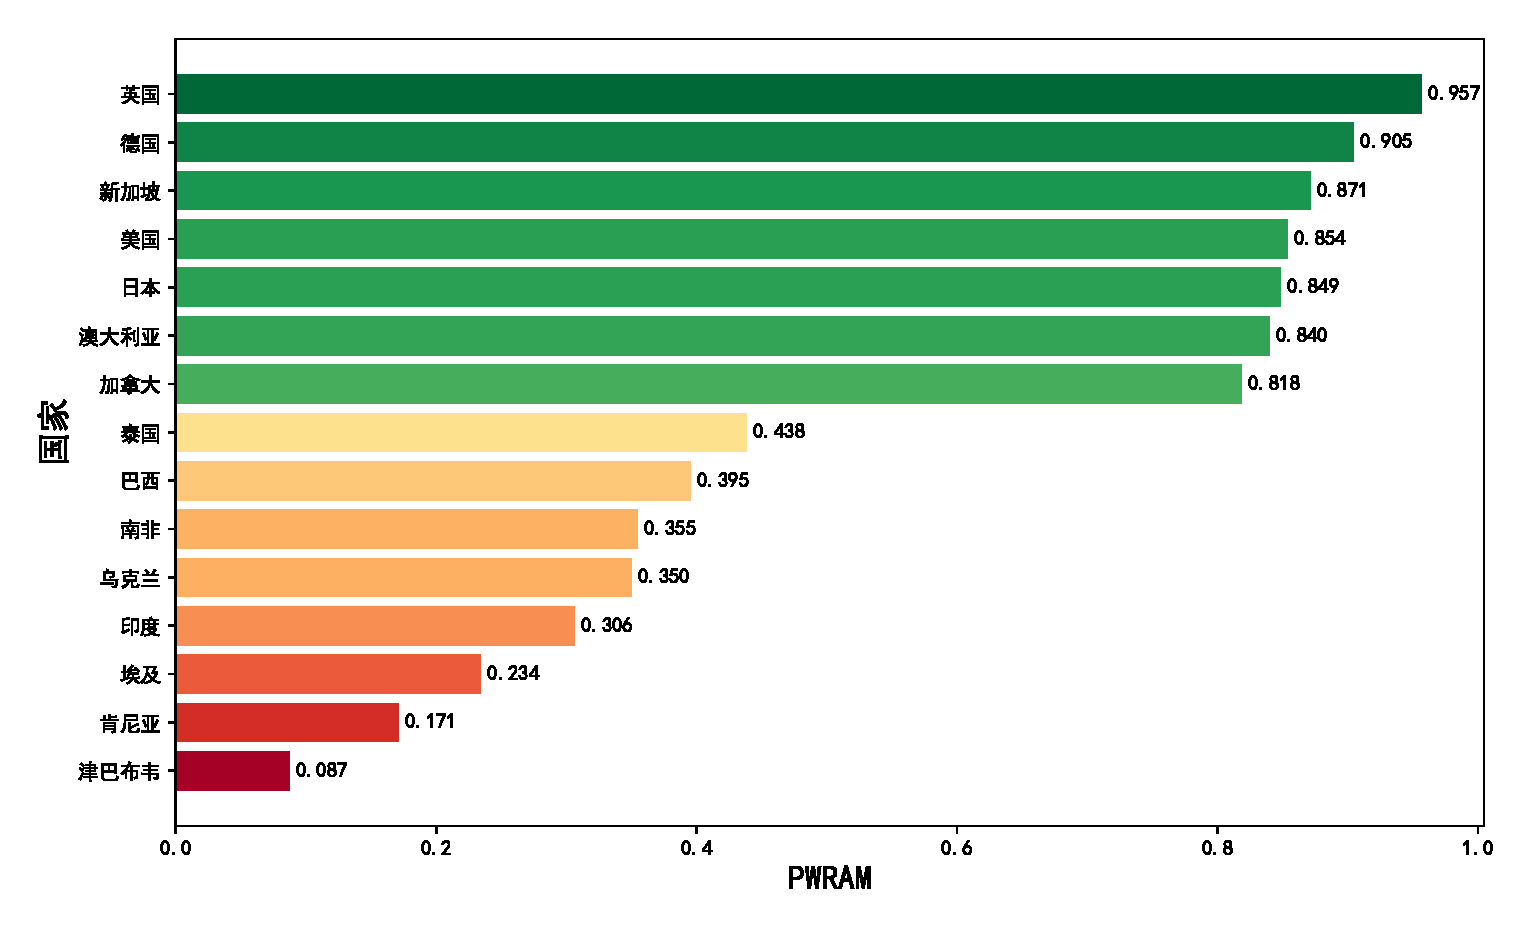
\includegraphics[width=0.8\textwidth]{figures/pwram.eps}
\caption{15个国家或地区的PWRAM模型结果}
\label{fig:pwram}
\end{figure}

\begin{figure}[h]
  \centering
  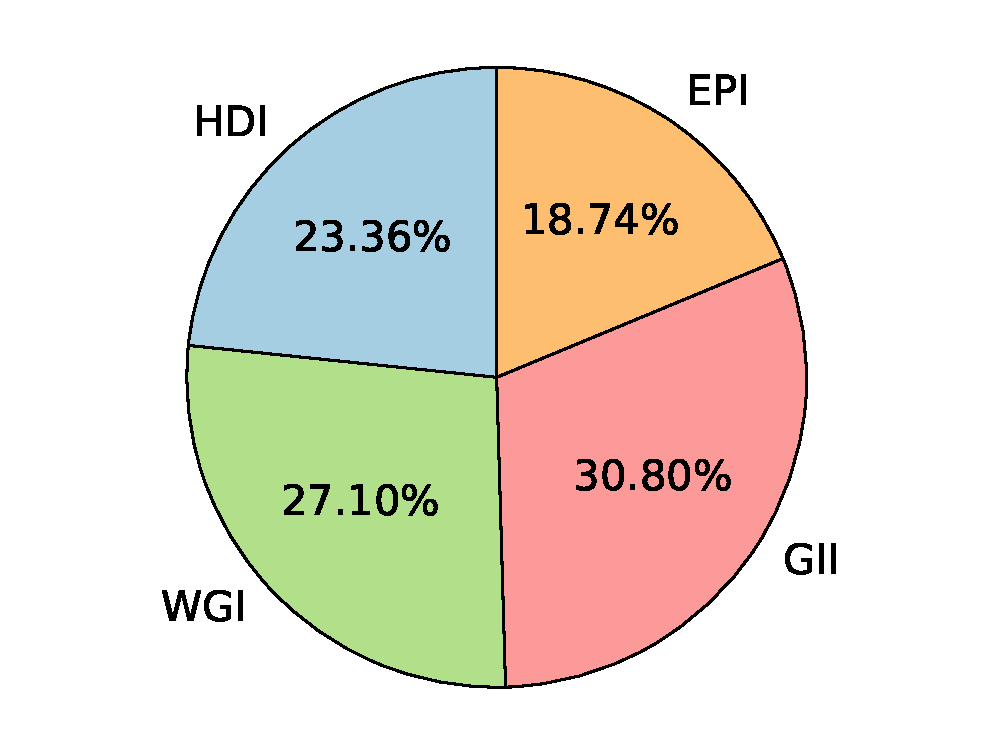
\includegraphics[width=0.5\textwidth]{weights}
  \caption{PWRAM模型在15个国家或地区样本集中的权重分布}
\end{figure}

\begin{figure}[h]
  \centering
  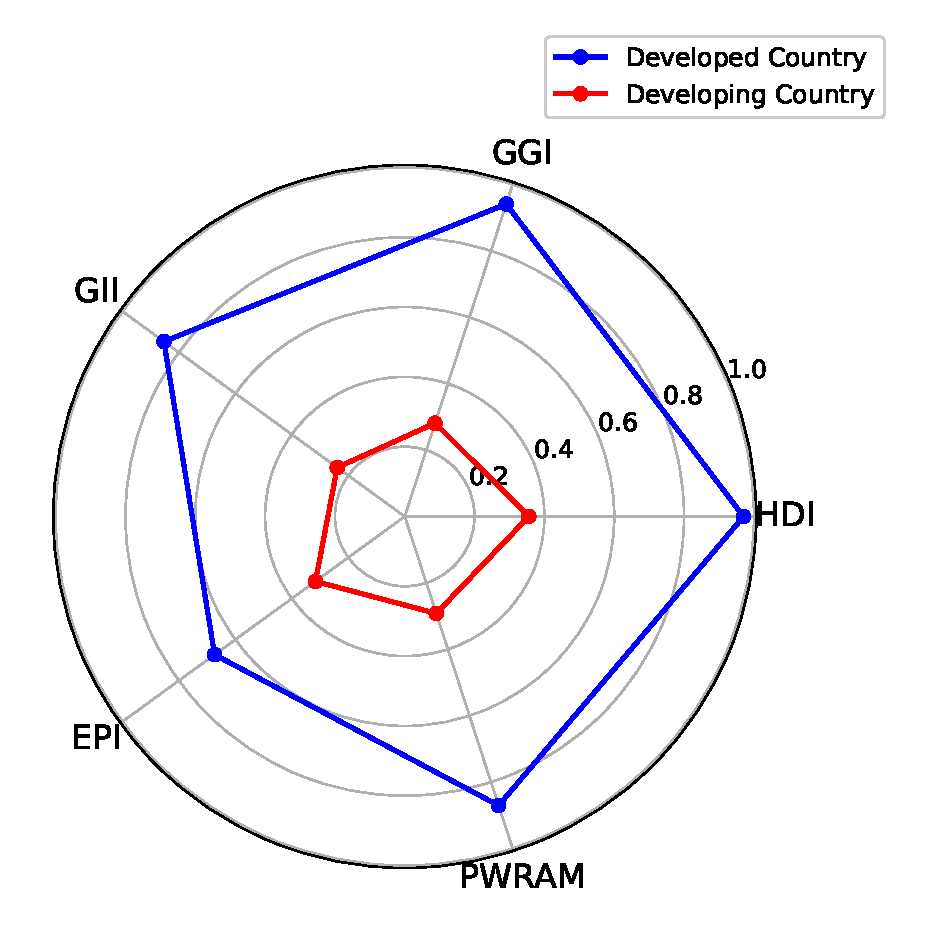
\includegraphics[width=0.5\textwidth]{radar}
  \caption{发达国家与发展中国家的PWRAM平均结果差异}
\end{figure}

\subsubsection{设定目标}

我们希望通过设置一个全球范围内的目标,即提高国家与地区的PWRAM水平,从而减少全球范围内的塑料制品浪费。根据我们PWRAM模型的评估结果,即图\ref{fig:pwram},我们可以看到,发达国家的塑料制品浪费减少能力较强,而发展中国家塑料制品浪费减少能力较弱。同时,如图\ref{fig:plastic-waste}所示\cite{owid-plastic-pollution},我们可以看到,海洋倾倒的塑料废物大部分来自发展中国家,这说明大部分\textit{管理不善}的塑料废物来自发展中国家。因此,我们期望为全球的发展中国家设定一个合理的PWRAM目标水平,从而保护全球环境,减少塑料制品浪费。

\begin{figure}[h]
\centering
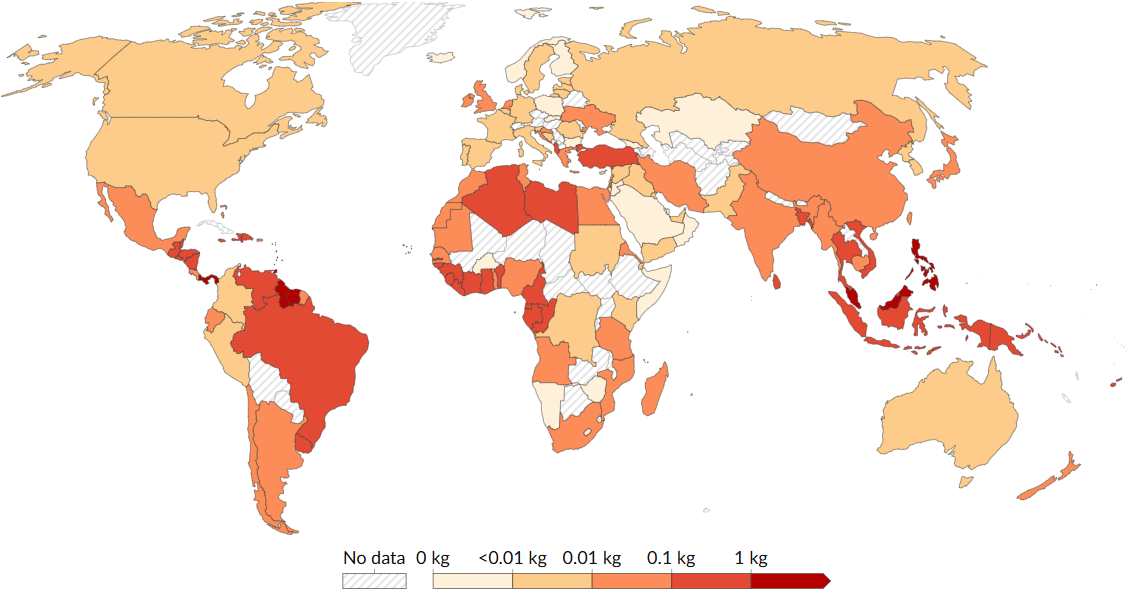
\includegraphics[width=0.8\textwidth]{plastic-waste}
\caption{2019年全球范围内的塑料废物海洋倾倒量(人均)}
\label{fig:plastic-waste}
\end{figure}

根据发达国家的数据以及发展中国家与发达国家之间的差距,我们认为PWRAM达到0.7时,可以有效减少塑料制品的浪费并达到一个环境安全的水平。为达到这一目标,我们可以通过以下几个方面来提高发展中国家的PWRAM水平:

\begin{itemize}
  \item HDI水平:提高人类发展指数,即提高国家与地区的经济水平。这取决于国家的经济政策与国际贸易环境,提升空间较小。对于发达国家来说,这一指标通常趋于稳定,而对于发展中国家来说,往往会保持一个较高的增长速度。因此,我们假设发展中国家的HDI水平可以以当前的平均增长速度增长,即每年增长0.7\%。
  \item WGI水平:提高全球治理指数,即提高国家与地区的政治水平。这取决于国家的政治体制与政府治理能力,对于发展中国家来说,这一指标通常较低,可干预空间较大。一般情况下,这一指标会长期稳定在一个较低的水平。我们假设在环球保护组织的支持下,减少塑料制品政策会相继出台,其实施力度会逐渐加大,在此基础上,WGI以每年增长1.0\%的速度增长。
  \item GII水平:提高全球创新指数,即提高国家与地区的科技水平。发展中国家的GII水平通常较低,可干预空间较大。发展中国家可以出台宏观政策,在国际社会的支持下,GII水平可以以一个约1.1\%稳定的速度增长。
  \item EPI水平:提高环境绩效指数,即改善环境水平。对于发展中国家来说,先污染后治理的现象较为普遍,因此EPI水平较低。如果发展中国家能够加大环境保护力度,发展绿色经济,由于环保绩效是缓慢提升的,我们参考近年来中国的环保成效,假设EPI水平可以以每年增长0.74个单位。
\end{itemize}

我们以发展中国家之一巴西为例,根据上述的增长速度,我们可以计算出经过30年的稳定发展与政策调控,最终巴西可以实现PWRAM水平达到0.7的目标水平,结果如图\ref{fig:bar}所示。

\begin{figure}[h]
\centering
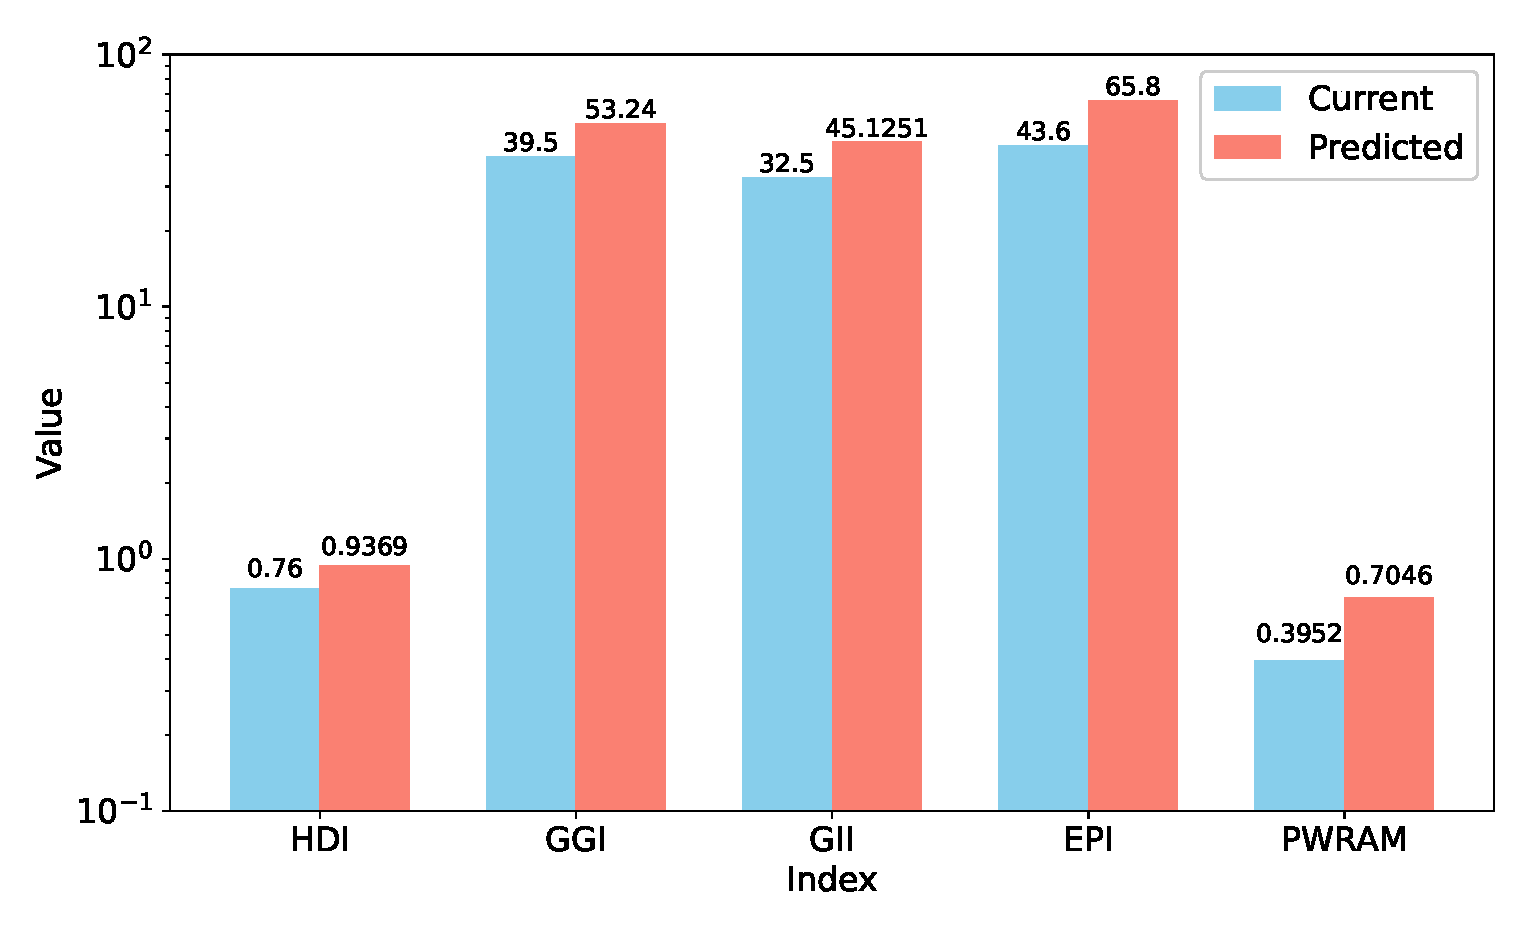
\includegraphics[width=0.8\textwidth]{bar}
\caption{巴西PWRAM模型预测结果}
\label{fig:bar}
\end{figure}

在实现这一目标之后,我们探讨其会造成的影响:

\begin{itemize}
  \item 对塑料业的影响:通过提高WGI水平,政府会出台更多强有力的环保政策,对塑料制品的生产、使用、回收等方面进行规范、限制,这对传统的塑料业会带来较大的冲击。同时,由于绿色产品政策的推动,生物可降解塑料等新型塑料制品的市场需求会逐渐增加,这将带动塑料业的转型升级。在提高GII水平的支持下,一系列新兴科技的应用将会进一步推动生物可降解塑料等新型塑料制品的研发与应用,从而推动塑料业的发展,为塑料业的可持续发展提供新的动力。
  \item 对生态环境的影响:通过提高WGI水平,政府会加大对环境保护的力度,一些环保政策的出台,如禁塑令、限塑令等,将会有效减少一次性塑料制品的使用,同时通过政策加强对塑料废物的处理与回收,最终能够有效减少塑料废物对环境的污染。在政策的推动下,环境保护意识会上升到教育层面,人们会更加重视环境保护,从而形成良好的环保氛围。环境的改善进一步正反馈提高了EPI水平,更高的环境承载力意味着更有效的塑料废物处理能力,形成了一个良性循环。
  \item 对人类生活的影响:通过提高WGI水平,政府会为绿色环保塑料产品提供相应的政策优惠,如减免税收、补贴等,这将有效降低绿色环保塑料产品的价格,提高人们购买绿色环保塑料产品的意愿,绿色健康产品会逐渐进入到人们的生活当中来;管理不善的塑料浪费量会逐渐减少,海洋内微塑料含量会趋于稳定,同时由于GII水平的提高,微塑料的处理技术会逐渐成熟,微塑料的处理效率会逐渐提高,从而避免微塑料经由食物链威胁到人类的健康,海洋产品将会更加安全,推动海洋市场的健康发展。
\end{itemize}

\subsection{公平性问题}

塑料垃圾危机是一个全球性的问题,与我们每一个人都息息相关。其成因虽然由不同的国家和地区所造成,但其影响需要全球范围内的国家与地区来共同承担。尽管如此,如图\ref{fig:pwram}所示,不同的国家与地区之间的PWRAM水平差距较大,发达国家的PWRAM水平较高,而发展中国家的PWRAM水平较低,而且分布较为不均衡。这种不均匀的分布主要是由于发达国家的经济水平有较大优势,而发展中国家的水平较低所造成的。

\begin{figure}[h]
  \centering
  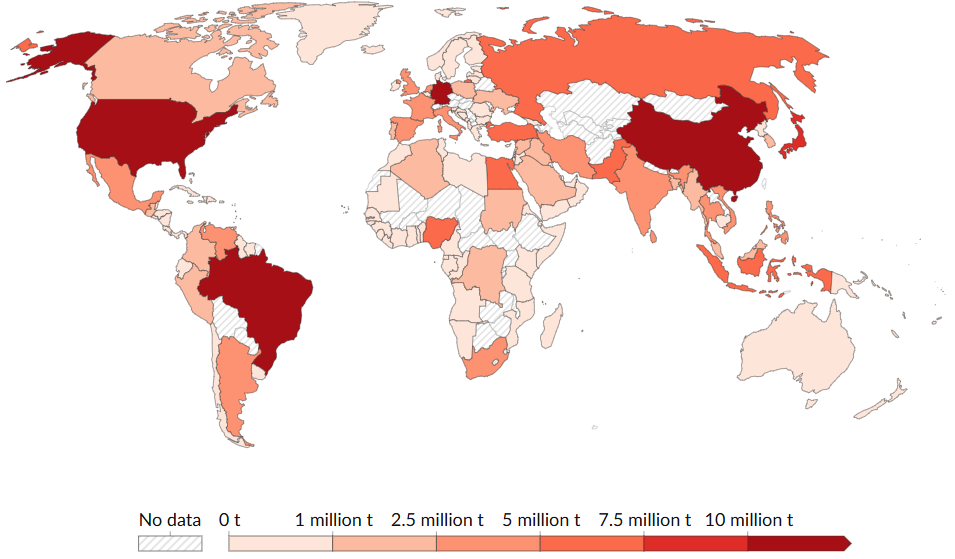
\includegraphics[width=0.75\textwidth]{prod}
  \caption{2010年各国塑料制品生产量(单位:百万吨)}
  \label{fig:prod}
\end{figure}

如图\ref{fig:prod}所示\cite{owid-plastic-pollution},虽然欧美发达国家的塑料制品生产量较高,但都有着较高的PWRAM水平,因此,塑料废物的生产与消耗形成了良性循环;相比之下,发展中国家的塑料制品生产量同样较高,但是这些国家的PWRAM水平较低,难以有效处理塑料废物,最终导致了大量塑料废物管理不善,对环境造成了严重的污染。因此,想要解决塑料垃圾危机,需要全球范围内的国家与地区共同努力,共同承担。

综上所述,我们建议PWRAM高水平梯队国家应当与PWRAM低水平梯队国家建立起\textbf{多边合作},开启全球范围内的塑料垃圾治理合作,发达国家可以提供技术支持、资金支持等,帮助发展中国家实施落实更有效的政策,提高其PWRAM水平,从而共同推动全球塑料垃圾治理事业的发展;发展中国家也可以通过其自身优势,与发达国家展开对话,实现合作共赢。

共同承担全球塑料垃圾治理的责任,才能共同推动全球塑料垃圾治理事业的发展。我们相信,只有全球范围内的国家与地区共同努力,才能有效解决塑料垃圾危机,保护全球环境,推动全球可持续发展。

\section{模型评价}

\subsection{模型的优点}

\begin{itemize}
  \item \textbf{综合性强}:我们的MSPWR模型考虑了塑料处理的各个途径,包括回收利用、焚烧处理、填埋处理,计算方式充分考虑到环境承载能力,形成的结果具有一定的可靠性;而PWRAM模型则弥补MSPWR模型的欠缺,还考虑了国家与地区的塑料废物处理能力,综合考虑了HDI、WGI、GII、EPI四个被国际广泛认可的指标,形成了一个较为全面的评估体系。
  \item \textbf{具有操作性}:我们从PWRAM模型的四个评价指标出发,提出了通过世界环保组织或发达国家的人为干预来提高发展中国家的WGI、GII水平等方面的具体解决方案。
  \item \textbf{公平性强}:我们的模型考虑了全球范围内的国家与地区之间的PWRAM水平差距,提出了多边合作的解决方案,具有较强的公平性。
  \item \textbf{模型敏感性}:由于我们的模型对于不同的国家与地区具有较高的敏感性,能够较好地反映不同国家与地区的PWRAM水平,这是因为我们的模型以HDI, WGI, GII, EPI四个指标为基础,对各个国家的经济、政策、环境因素的变化具有较高的敏感性,由于这些数据经过熵权法的处理,因此任一指标的变化都会对最终的PWRAM水平产生影响。
\end{itemize}

\subsection{模型的不足}

\begin{itemize}
  \item \textbf{数据样本较小}:我们的模型在计算PWRAM水平时,使用了全球范围内15个国家或地区的HDI、WGI、GII、EPI的数据,囊括了发达国家、发展中国家和欠发达国家,虽然这些数据具有一定的代表性,但是仍然不足以覆盖全球范围内的所有国家与地区,因此模型的普适性有待提高。
  \item \textbf{模型预测精确度}:我们的模型在设定目标时,以巴西为例,得出了巴西可以在30年内实现 PWRAM 水平达到0.7的目标水平,这种预测有一定的参考价值,但是由于\textbf{近年来疫情、经济下行}等因素的影响,这种预测仍然存在一定的不确定性。
\end{itemize}


\section{结论}

在我们的文章中,我们通过提出两个数学模型(MSPWR,PWRAM)为全球塑料垃圾危机贡献了治理方案。我们首先分析了塑料垃圾危机的处理方式,建立了MSPWR模型,利用国家所发布的碳排放数据可以粗略估计出可以安全减轻的一次性或一次性使用的塑料产品浪费的最大量。然后,我们建立了PWRAM模型,通过对15个国家或地区的HDI、WGI、GII、EPI的数据进行归一化处理,计算了这些国家或地区的PWRAM水平。我们通过设定目标,提出了一系列的解决方案,包括提高WGI、GII水平等方面,最终实现了巴西可以在30年内实现PWRAM水平达到0.7的目标水平。我们还分析了这一目标的影响,包括对塑料业、生态环境、人类生活等方面的影响。最后,我们提出了多边合作的解决方案,期望全球国家能够共同承担全球塑料垃圾治理的责任,共同推动全球塑料垃圾治理事业的发展。

\bibliography{add}

\newpage

\begin{appendices}

\section{Memo}

TO: ICM

FROM: 武泽恺

DATE: \today

SUBJECT: 关于全球塑料垃圾危机治理方案的研究报告

\begin{letter}{尊敬的评委:}

在探讨全球塑料垃圾危机的治理方案时,我们提出了两个创新的数学模型:MSPWR( Maximum Single-Use Plastic Waste Reduction )和PWRAM( Plastic Waste Reduction Ability Model )。以下是我们研究的主要发现和提出的解决方案。

\begin{figure}[h]
  \centering
  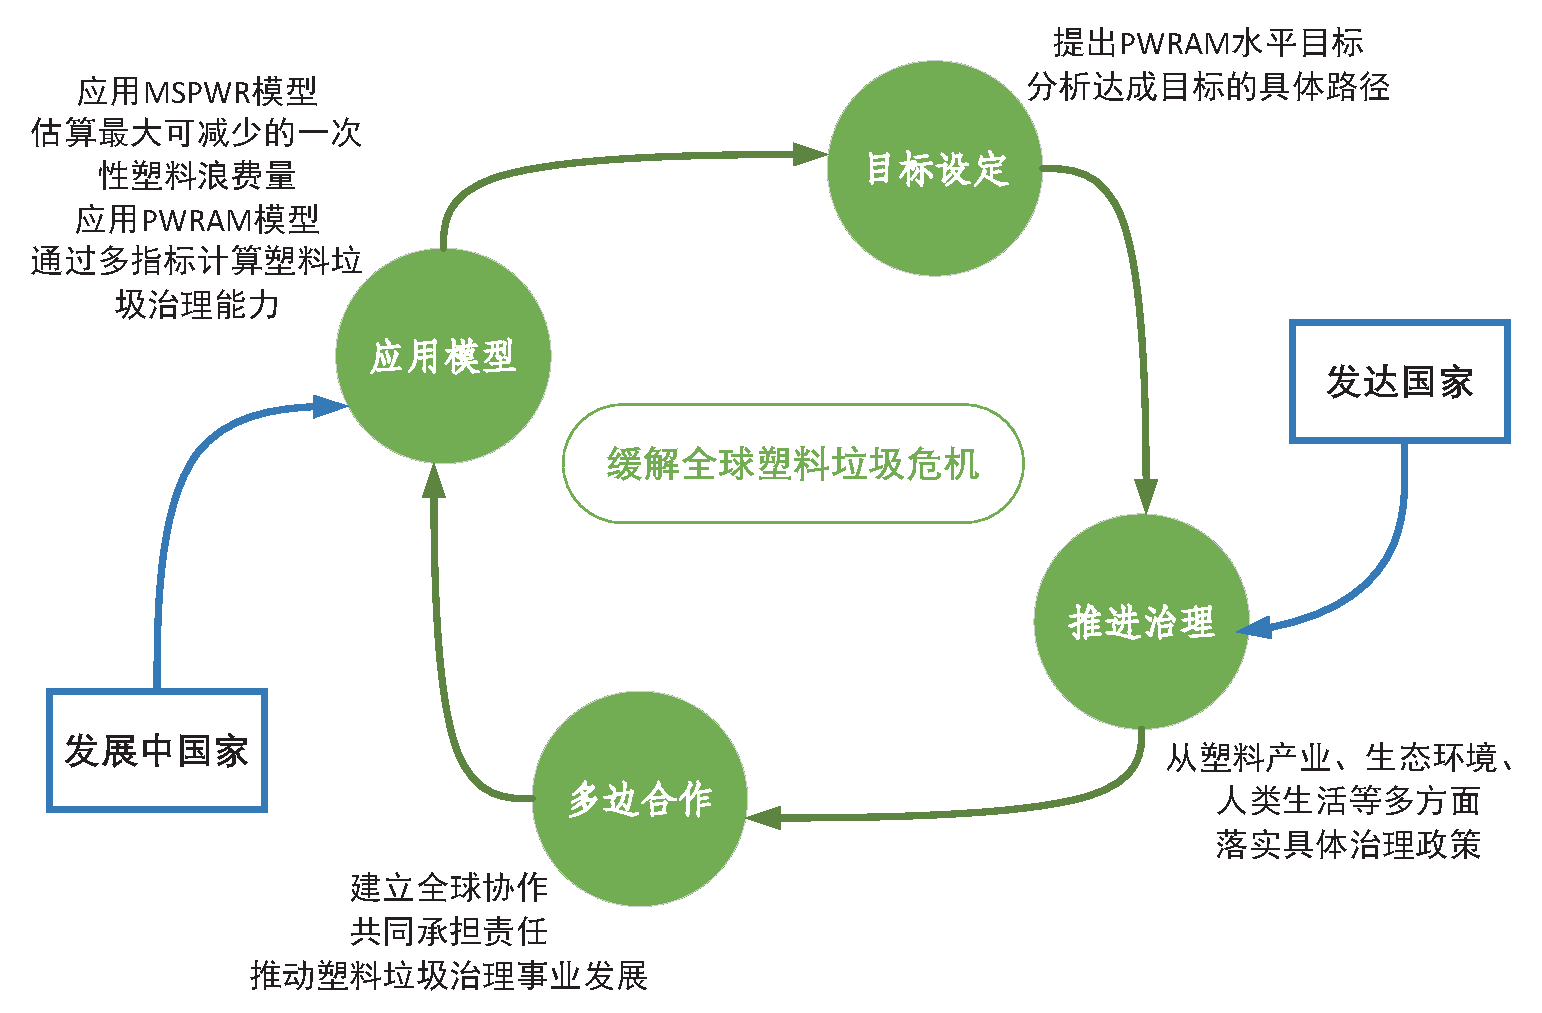
\includegraphics[width=0.8\textwidth]{figures/framework.eps}
  \caption{全球塑料垃圾治理框架}
  \label{fig:framework}
\end{figure}

我们的研究首先分析了塑料垃圾危机的处理方式,通过建立MSPWR模型,利用各国发布塑料回收比例、可降解塑料产量、$\text{CH}_4$排放数据和$\text{CO}_2$排放数据,我们能够粗略估计出可以安全减轻的一次性或一次性使用的塑料产品浪费的最大量。这一模型为全球塑料垃圾减排提供了一个初步的理论框架,帮助各国根据自身的碳排放情况,确定塑料减排的最大安全阈值。

随后,我们构建了PWRAM模型,通过对15个国家或地区的人类发展指数(HDI)、全球治理指标(WGI)、全球创新指数(GII)、环境绩效指数(EPI)的数据进行归一化处理,计算了这些国家或地区的PWRAM水平。这一模型可以有效评估各国在塑料垃圾减排方面的能力,为全球塑料垃圾治理提供了一个科学的评估体系。

同时,我们还为发展中国家设定了一个目标,并提出了一系列解决方案,包括提高WGI、GII水平等方面,以促进全球塑料垃圾的有效减排。我们的研究表明,巴西等国家有望在 30 年内实现PWRAM水平达到0.7的目标水平。实现这一目标,可以对塑料业、生态环境、人类生活产生深远影响,包括促进塑料产业的绿色转型、改善生态环境质量、提升人类生活质量等。

最后,由于各国的塑料减排能力不尽相同,我们强调了多边合作的重要性。我们期望全球国家能够共同承担全球塑料垃圾治理的责任,通过共享技术、资金和最佳实践,共同推动全球塑料垃圾治理事业的发展。我们提出的多边合作解决方案包括建立国际合作机制、推动技术创新、加强环境教育和公众参与等。

希望我们的研究为全球塑料垃圾危机提供了有效的解决方案,我们也希望全球合作能够在塑料垃圾治理中发挥关键作用。我们相信,通过各国的共同努力,我们能够实现塑料垃圾的有效减排,保护我们的地球家园。  

\vspace{\parskip}

此致

敬礼

武泽恺

\end{letter}

\newpage

\section{拟合可降解塑料产量数据代码}
\label{sec:fit}

\lstinputlisting[language=python]{./code/fit.py}

\section{PWRAM模型代码}
\label{sec:pwram}

\lstinputlisting[language=python]{./code/pwram.py}

\end{appendices}

\AImatter

\begin{ReportAiUse}{9}
\bibitem{AI1}
ChatGPT\\
Query1: 综合指数公式一般有哪些形式?\\
Output: 综合指数的构建通常基于不同的目标和特性,可以采用多种形式来表达。以下是几种常见的综合指数模型形式:

1. 线性加权模型
这是最常见的综合指数形式,权重与各项指标直接相乘后加和:
\[
I = \sum_{i=1}^n w_i \cdot x_i
\]
- 特点:简单直观,易于计算和解释。
- 适用场景:指标之间相互独立且没有非线性关系时。
- 关键点:权重 \( w_i \) 的确定方式可以基于主观判断(如专家评分)或客观方法(如熵权法、回归分析)。


2. 几何加权模型
通过指标的乘积计算综合指数:
\[
I = \prod_{i=1}^n x_i^{w_i}
\]
- 特点:用于捕捉指标间的相互作用。当某一指标趋近 0 时,综合指数显著降低。
- 适用场景:强调“短板效应”,即某些关键指标过低会显著拉低整体水平。
- 关键点:权重 \( w_i \) 控制每个指标对综合指数的贡献。

3. 非线性加权模型
通过非线性函数对指标进行变换:
\[
I = f\left(\sum_{i=1}^n w_i \cdot x_i^k \right)
\]
其中,\( k \) 是非线性系数,\( f \) 是映射函数(如指数函数、对数函数等)。
- 特点:可以调整指标的敏感性,适应复杂的非线性关系。
- 适用场景:指标对综合指数的影响并非线性(如环境模型中碳排放的非线性效应)。
- 关键点:选择合适的非线性函数和参数 \( k \)。

4. 模糊综合评判模型
基于模糊数学理论,将多个指标模糊化后得到综合评价结果:
\[
I = W \cdot R
\]
其中:
- \( W \) 是权重向量;
- \( R \) 是指标的模糊矩阵。
- 特点:适合处理模糊和不确定性信息。
- 适用场景:数据不精确或需要考虑主观判断(如社会满意度调查)。
- 关键点:需要定义模糊隶属函数。

5. 主成分分析模型
利用统计方法提取原始指标的主要特征:
\[
I = \sum_{i=1}^k a_i \cdot PC_i
\]
其中,\( PC_i \) 是第 \( i \) 个主成分,\( a_i \) 是主成分的权重。
- 特点:减少维度,避免指标的多重共线性问题。
- 适用场景:指标高度相关、数据维度较高时。
- 关键点:解释主成分的含义,确保其具有实际意义。

6. 熵权模型
通过熵值确定指标的权重,计算公式为:
\[
I = \sum_{i=1}^n w_i \cdot x_i \quad \text{其中} \quad w_i = \frac{d_i}{\sum_{j=1}^n d_j}, \, d_i = 1 - H_i
\]
- 特点:自动确定权重,减少主观干扰。
- 适用场景:指标数据较多且权重难以直接确定时。
- 关键点:需保证数据标准化,并理解熵值的物理意义。

7. TOPSIS 模型
基于多指标距离评价,计算每个方案与理想方案的距离:
\[
I = \frac{S^-}{S^+ + S^-}
\]
其中:
- \( S^+ \) 是与正理想解的距离;
- \( S^- \) 是与负理想解的距离。
- 特点:综合考虑指标与理想目标的接近程度。
- 适用场景:指标有正负向性,且需要综合排序时。
- 关键点:需要标准化数据和定义理想解。

8. AHP 层次分析模型
通过构建层次结构和成对比较矩阵,得到权重:
\[
I = \sum_{i=1}^n w_i \cdot x_i
\]
- 特点:结合主观和客观判断,适用于多级指标综合评价。
- 适用场景:指标层次复杂且需专家意见支持时。
- 关键点:确保成对比较矩阵的一致性。

选择模型的考虑因素
1. 指标特性:指标是否独立,是否存在线性关系。
2. 数据质量:数据的完整性、准确性及是否需要标准化处理。
3. 计算复杂度:根据实际应用选择合适的复杂度。
4. 适用场景:例如短板效应适合几何模型,模糊环境适合模糊综合评判。

以上模型可以单独使用或结合实际问题进行组合应用,满足具体需求。

\end{ReportAiUse}

\end{document}
%% 
%% This work consists of these files mcmthesis.dtx,
%%                                   figures/ and
%%                                   code/,
%% and the derived files             mcmthesis.cls,
%%                                   mcmthesis-demo.tex,
%%                                   README,
%%                                   LICENSE,
%%                                   mcmthesis.pdf and
%%                                   mcmthesis-demo.pdf.
%%
%% End of file `mcmthesis-demo.tex'.
